\let\negmedspace\undefined
\let\negthickspace\undefined
\documentclass[journal]{IEEEtran}
\usepackage[a5paper, margin=10mm, onecolumn]{geometry}
%\usepackage{lmodern} % Ensure lmodern is loaded for pdflatex
\usepackage{tfrupee} % Include tfrupee package

\setlength{\headheight}{1cm} % Set the height of the header box
\setlength{\headsep}{0mm}     % Set the distance between the header box and the top of the text

\usepackage{gvv-book}
\usepackage{gvv}
\usepackage{cite}
\usepackage{amsmath,amssymb,amsfonts,amsthm}
\usepackage{algorithmic}
\usepackage{graphicx}
\usepackage{textcomp}
\usepackage{xcolor}
\usepackage{txfonts}
\usepackage{listings}
\usepackage{enumitem}
\usepackage{mathtools}
\usepackage{gensymb}
\usepackage{comment}
\usepackage[breaklinks=true]{hyperref}
\usepackage{tkz-euclide} 
\usepackage{listings}
% \usepackage{gvv}                                        
\def\inputGnumericTable{}                                 
\usepackage[latin1]{inputenc}                                
\usepackage{color}                                            
\usepackage{array}                                            
\usepackage{longtable}                                       
\usepackage{calc}                                             
\usepackage{multirow}                                         
\usepackage{hhline}                                           
\usepackage{ifthen}                                           
\usepackage{lscape}
\begin{document}

\bibliographystyle{IEEEtran}
\vspace{3cm}

\title{9-9.2-38}
\author{AI24BTECH11002 - K.AKSHAY TEJA}
% \maketitle
% \newpage
% \bigskip
{\let\newpage\relax\maketitle}

\renewcommand{\thefigure}{\theenumi}
\renewcommand{\thetable}{\theenumi}
\setlength{\intextsep}{10pt} % Space between text and floats


\numberwithin{equation}{enumi}
\numberwithin{figure}{enumi}
\renewcommand{\thetable}{\theenumi}


\textbf{Question}:\\
Find the area bounded by the curve $y = x|x|, x$-axis and the ordinates $x=-1$ and $x=1$.


 \solution
 \begin{table}[h!]
 	\centering
 	\begin{tabular}{|c|c|}
	\hline
	Vector&Description\\
	\hline
	Vector A&  \(\hat{i} - 2 \hat{j} + 3 \hat{k}\)\\
	\hline
	Vector B& \(2\hat{i} +3 \hat{j} -4\hat{k}\)\\
	\hline
	Vector C& \(\hat{i} -3\hat{j} +\hat{k}\)\\
	\hline
\end{tabular}

 	\caption{Information}
 	\label{tab:9-9.2-38}
 \end{table}

For $x\geq0$, the equation of the curve is given by 
\begin{align}
    y = x^2
\end{align}
For $x<0$, the equation of the curve is given by 
\begin{align}
    y = -x^2
\end{align}
As you can see in the figure, the area bounded by the curve $y = x|x|$ in between the lines $x = -1$ and $x = 1$ is given by
\begin{align}
	\int_{-1}^{0} \abs{-x^2}dx + \int_{0}^{1} \abs{x^2}dx = \frac{2}{3} 
\end{align}
 \begin{figure}[h!]
 \begin{center}
 	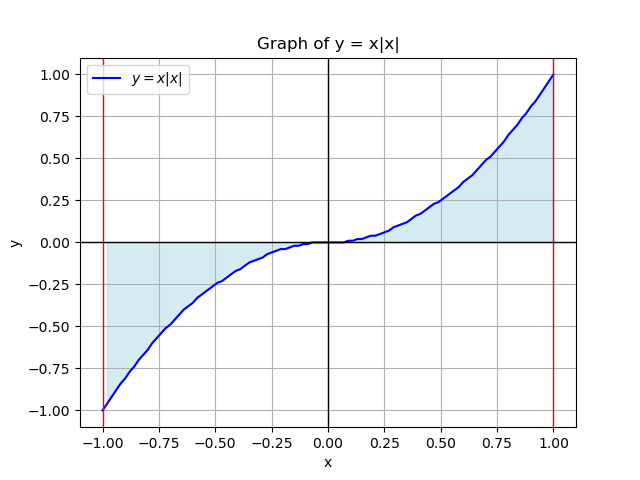
\includegraphics[width=0.635\textwidth]{Fig/fig.png}
 	\caption{Graph of $ y = x|x|$}
 	\label{fig:9-9.2-38 - Figure -1}
 \end{center}
 \end{figure}
\end{document}




